\newgeometry{
	textwidth = 134 mm,
    textheight = 220 mm, 
    top = 38 mm,
    inner = 38 mm,
}
\begin{titlepage}
    \sffamily
    % background picture
	%\begin{tikzpicture}[overlay, remember picture]
	%\node[anchor=north east, 
	%	xshift=+0.2cm, 
	%	yshift=+0.2cm] 
	%	at (current page.north east)
	%	{\includegraphics[width = 1.52\linewidth]{images/cover}};%titelbild 
	%\end{tikzpicture}
	%\vspace*{14\baselineskip}

    \begin{center}
        %\includegraphics[height = 3.2 cm]{images/cover.pdf} \hfill 
\includegraphics[height = 3 cm]{images/Logo/Logo3.pdf}\\
        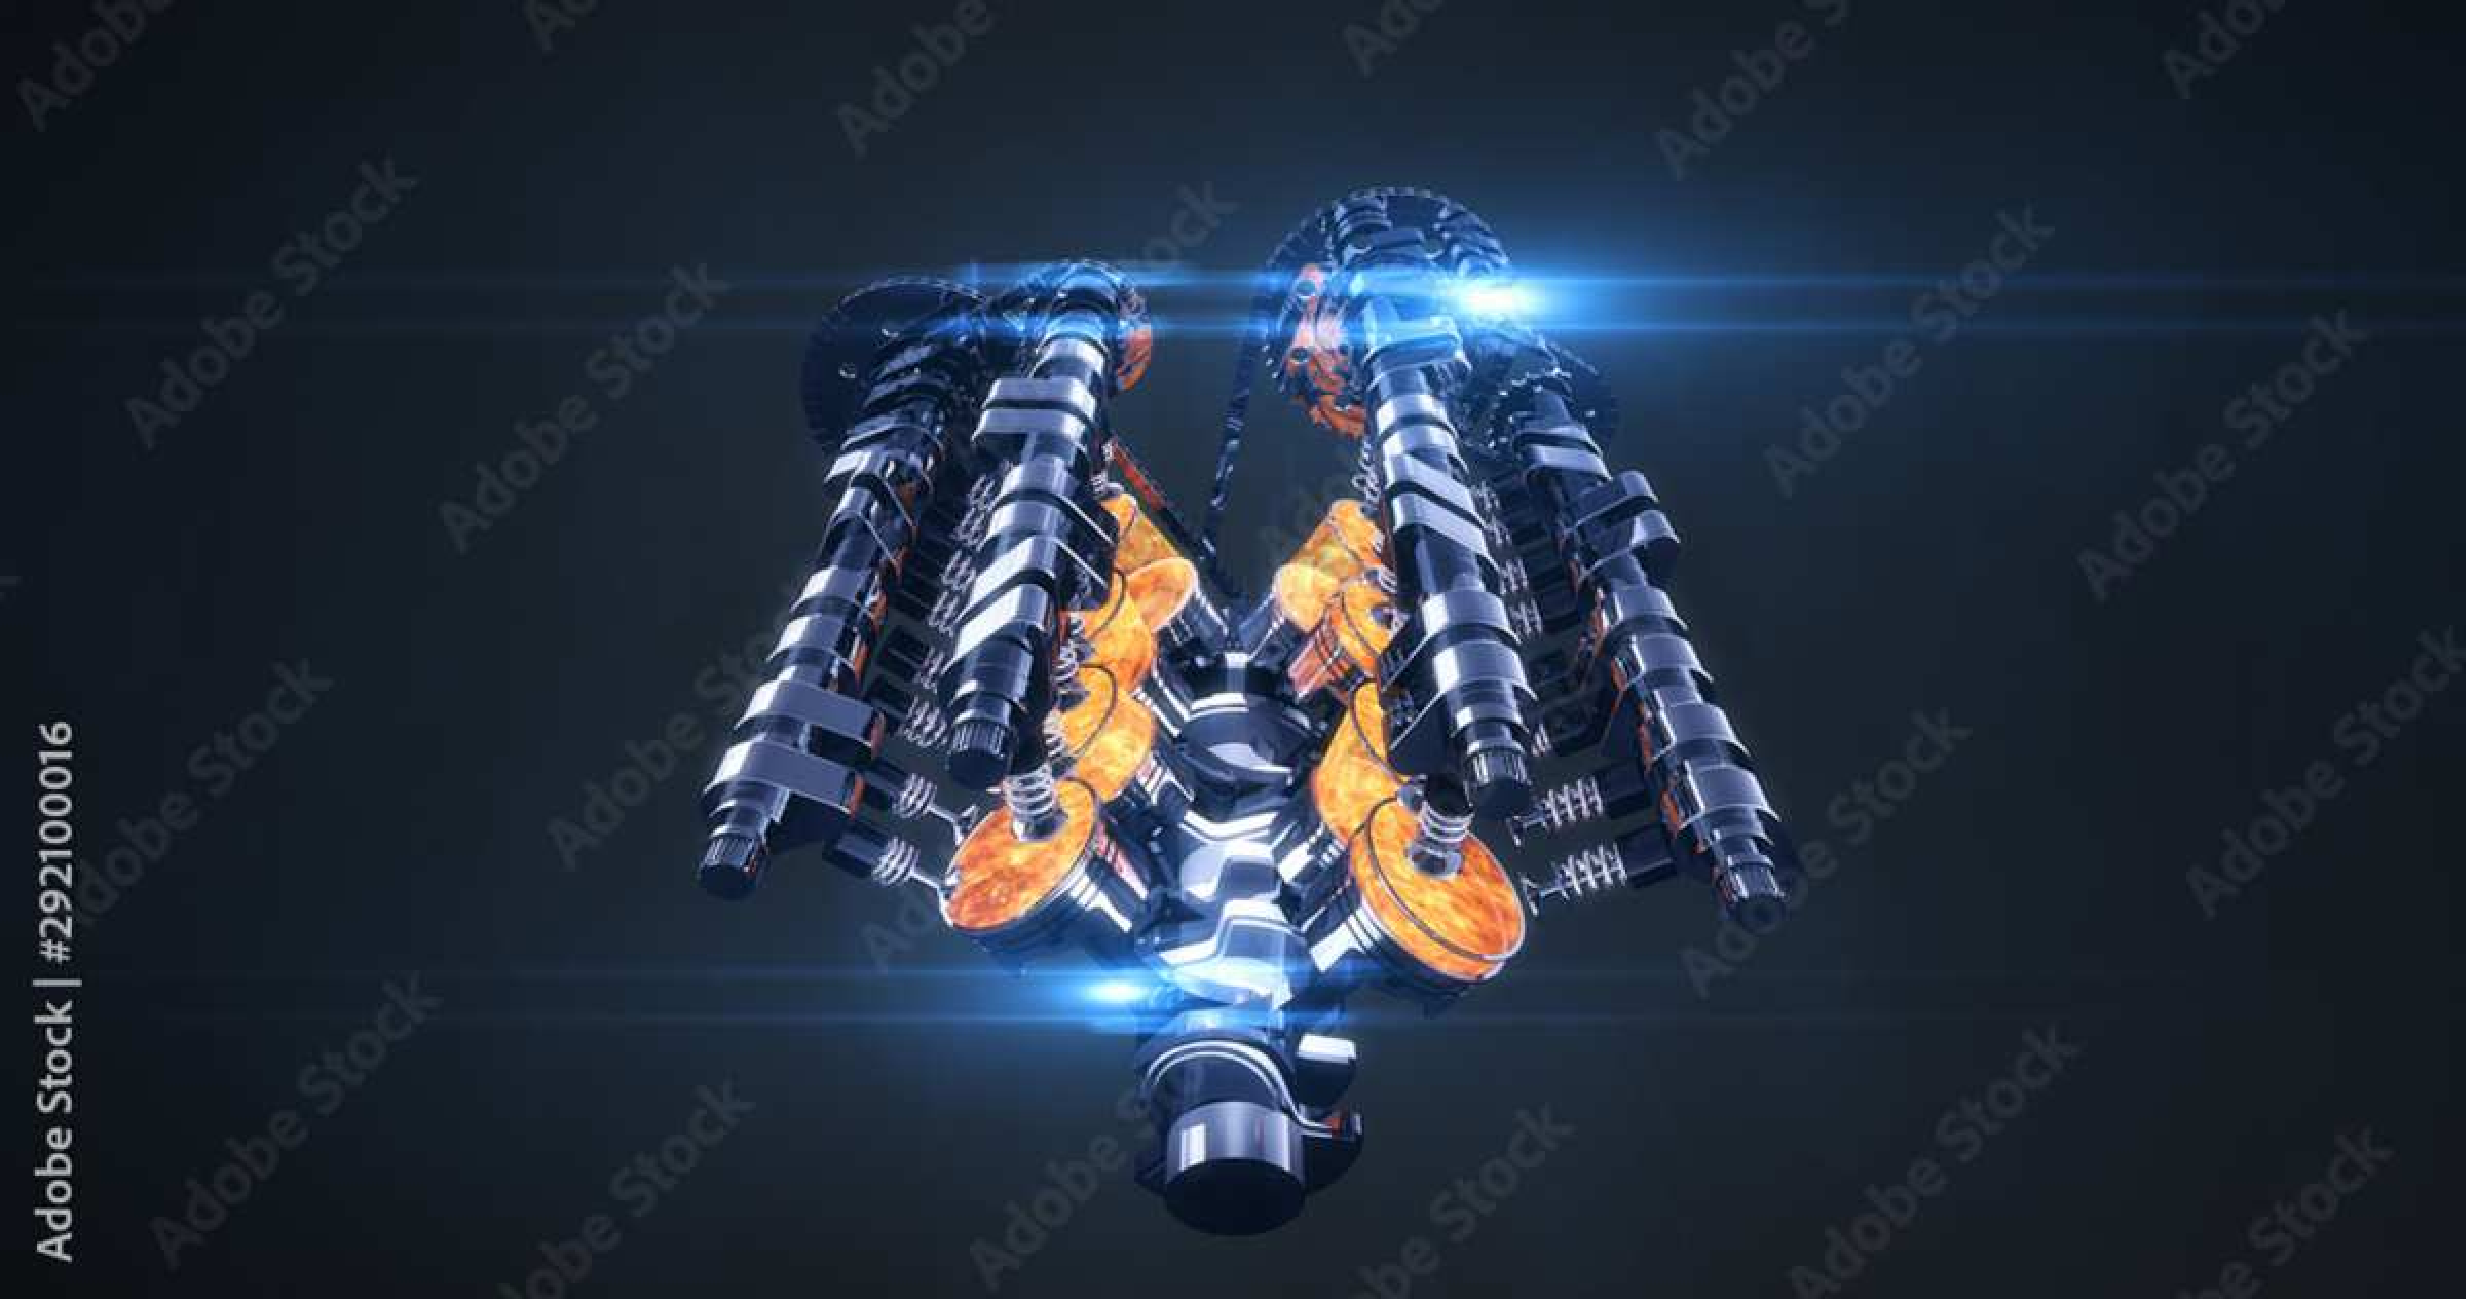
\includegraphics[width=\linewidth]{images/verbrennungsmotor.pdf}\\
        \vfil
        {\LARGE
            \rule[1 ex]{\textwidth}{1.5 pt}
            \thema\\[1 ex]
            {\vspace*{-1 ex}\Large \typ}\\
            \rule[-1 ex]{\textwidth}{1.5 pt}
        }
        \vfil
        {\Large\textbf{\name}}
        \vfil
        \bigskip
        \vfil
        {\large Version: \today \\[0.25 ex]}
    \end{center}
    
    \vfil
    \begin{table}[h]
        \centering
        \large
        \sffamily 
        {\def\arraystretch{1.2}
            \begin{tabular}{>{\bfseries}p{3.8 cm}p{5.3 cm}}
                Quelle                  & \quelle\\
            \end{tabular}
        }
    \end{table}
\end{titlepage}
\restoregeometry